% !TeX program = xelatex
% !TeX encoding = UTF-8
% Compile from this directory, or run build.ps1 from any directory.
\RequirePackage{iftex}
\RequireXeTeX
\makeatletter
\def\input@path{{../ieice_template/}}
\makeatother
\documentclass[letter]{ieice}

\usepackage{graphicx,xcolor}
\usepackage[fleqn]{amsmath}
\usepackage{tikz}
\usetikzlibrary{arrows.meta}
\usepackage{newtxtext}
\usepackage[varg]{newtxmath}
\usepackage{xeCJK}
\setCJKmainfont[
  BoldFont=FandolSong-Bold.otf,
  ItalicFont=FandolKai-Regular.otf
]{FandolSong-Regular.otf}
\setCJKsansfont[BoldFont=FandolHei-Bold.otf]{FandolHei-Regular.otf}
\setCJKmonofont{FandolFang-Regular.otf}

\usepackage[noadjust]{cite}
\renewcommand{\citepunct}{],\,\allowbreak[}
\renewcommand{\citedash}{]--\allowbreak[}
\makeatletter
\let\hyper@nopatch@caption\@empty
\makeatother
\usepackage{xurl}
\usepackage[hidelinks,hyperfootnotes=false]{hyperref}

\begin{document}
\pagestyle{plain}
% Keep natural heading and paragraph spacing; leave spare space at column bottoms.
\raggedbottom
\begin{summary}
本文结合 Tamarin、TLA$^{+}$ 形式化分析与参考实现实验，研究 AI Agent 安全架构 SAGA 的授权机制。研究发现，本应被拒绝的发送方能够获得访问控制令牌；获准通信的发送方在 OTK 领取额度耗尽后，仍可利用转交的 OTK 获取新令牌；同一令牌的并发使用可使超出授权额度的请求得到处理。
\end{summary}
\begin{keywords}
AI Agent，SAGA，形式化分析，访问控制，协议安全
\end{keywords}

% !TeX root = main.tex
% !TeX program = xelatex
% Introduction follows the analysis scope and evidence in Chapters 2--5.

\section{引言}
\label{sec:introduction}

在多代理系统中，代理间通信需要验证通信双方的身份，并限制通信建立及后续请求的执行。SAGA~\cite{syros2025saga} 是一种面向 AI Agent 系统的安全架构，通过接触策略决定发送方能否取得接收方的一次性公钥（One-Time Key，OTK），并由接收方利用 OTK 签发访问控制令牌（Access Control Token，ACT）。后续请求则由 ACT 的身份绑定、有效期和剩余请求额度进行控制。

SAGA 原有研究采用 ProVerif~\cite{blanchet2016proverif} 对代理与 Provider 之间的通信认证、代理间通信认证以及 ACT 机密性进行了形式化分析~\cite{syros2025saga}。然而，通信认证与 ACT 机密性并不足以保证授权机制的正确执行。代理间通信还受到接触策略、OTK 发放与使用以及 ACT 请求额度的限制，因此有必要进一步分析这些授权机制在协议执行过程中的安全性。

本文依据 SAGA 的协议规范与参考实现~\cite{syros2025sagaV2,sagaReferenceImpl2026}，采用 Tamarin~\cite{meier2013tamarin} 对接触策略匹配及 OTK 发放与使用进行形式化分析，采用 TLA$^{+}$~\cite{lamport2002specifying} 对 ACT 并发请求额度进行建模与验证，并结合参考实现实验开展安全分析。主要研究发现如下：

（1）接触策略匹配函数未能正确选择最匹配的规则，使本应被拒绝的发送方能够获得 ACT。

（2）OTK 未与领取者身份绑定，使获准通信的发送方在自身 OTK 领取额度耗尽后，仍可使用其他发送方领取并转交的 OTK 获得新的 ACT。

（3）ACT 有效性检查与额度扣减未在同一原子操作内完成，使同一 ACT 的并发使用可能导致接收方处理的请求数超过 ACT 的初始请求额度。


% !TeX root = main.tex
% !TeX program = xelatex
% Include this chapter with \input from an IEICE master document.
% Chinese draft compilation requires XeLaTeX and xeCJK in the master preamble.
% Bibliography entries are maintained in paper_letter/references.bib.

\section{授权流程与分析目标}
\label{sec:authorization-workflow-objectives}

\subsection{授权流程}
\label{subsec:authorization-workflow}

SAGA 的授权流程如图~\ref{fig:saga-authorization-workflow} 所示。设 Provider 为 $P$，接收方和发送方代理分别为 $A$ 和 $B$，两者均已完成注册与身份绑定。

\begin{figure}[tb]
  \centering
  % !TeX root = saga_authorization_compact.tex
% Normal successful path, at native publication size: 80 mm x 95 mm.
% Symbols: k is A's OTK public key, t the encrypted ACT, K a local shared key.
% Source: SAGA v2 IV-D2/IV-E and saga/{agent.py,provider/provider.py}.
% K is never transmitted. No atomicity or original-retriever binding is implied.
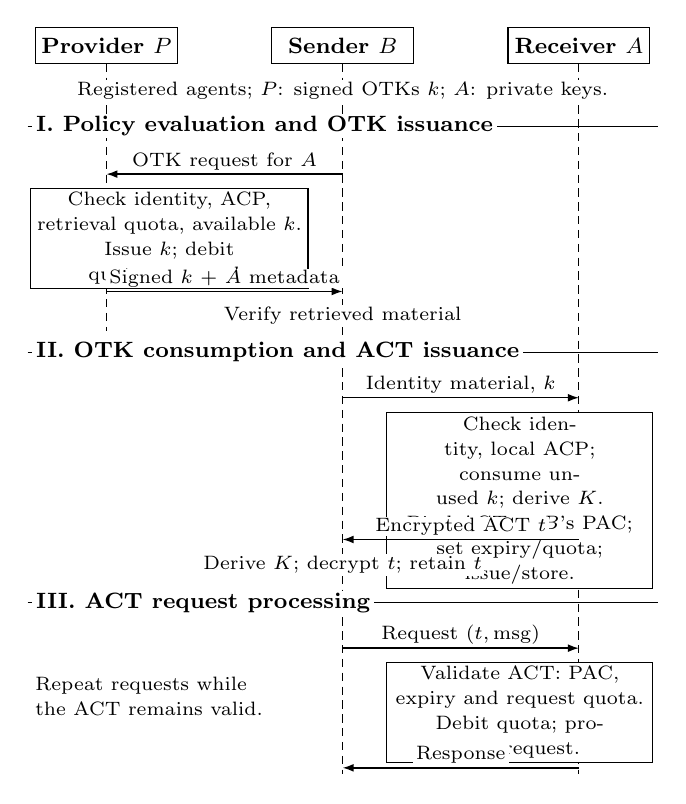
\begin{tikzpicture}[
  x=1mm,y=-1mm,
  font=\fontsize{7.5}{9}\selectfont,
  actor/.style={draw=black,line width=0.4pt,fill=white,
    minimum width=18mm,minimum height=4.6mm,inner sep=0pt,
    font=\bfseries\fontsize{8}{9.2}\selectfont},
  life/.style={draw=black,densely dashed,line width=0.4pt},
  msg/.style={-{Latex[length=1.4mm,width=1mm]},line width=0.5pt},
  wire/.style={fill=white,inner xsep=0.4mm,inner ysep=0.15mm},
  local/.style={draw=black,line width=0.4pt,fill=white,
    align=center,inner xsep=0.6mm,inner ysep=0.55mm,anchor=north},
  senderstep/.style={fill=white,align=center,inner sep=0.3mm},
  phase/.style={anchor=west,fill=white,inner xsep=0.5mm,
    inner ysep=0.2mm,font=\bfseries\fontsize{8}{9.2}\selectfont}
]
  \path[use as bounding box] (0,0) rectangle (80,95);
  \draw[life] (10,4.6) -- (10,38.5);
  \draw[life] (40,4.6) -- (40,94.8);
  \draw[life] (70,4.6) -- (70,94.8);
  \node[actor] at (10,2.3) {Provider $P$};
  \node[actor] at (40,2.3) {Sender $B$};
  \node[actor] at (70,2.3) {Receiver $A$};
  \node[fill=white,inner sep=0.2mm] at (40,8)
    {Registered agents; $P$: signed OTKs $k$; $A$: private keys.};

  \draw[line width=0.4pt] (0,12.5) -- (80,12.5);
  \node[phase] at (0.5,12.5) {I. Policy evaluation and OTK issuance};
  \draw[msg] (40,18.6) -- node[wire,above=0.3mm]
    {OTK request for $A$} (10,18.6);
  \node[local,text width=34mm] at (18,20.3) {
    Check identity, ACP,\\
    retrieval quota, available $k$.\\
    Issue $k$; debit quota; remove $k$.
  };
  \draw[msg] (10,33.5) -- node[wire,above=0.3mm]
    {Signed $k$ + $A$ metadata} (40,33.5);
  \node[senderstep] at (40,36.6) {Verify retrieved material};

  \draw[line width=0.4pt] (0,41.2) -- (80,41.2);
  \node[phase] at (0.5,41.2) {II. OTK consumption and ACT issuance};
  \draw[msg] (40,47) -- node[wire,above=0.3mm]
    {Identity material, $k$} (70,47);
  \node[local,text width=32.6mm] at (62.5,48.8) {
    Check identity, local ACP;\\
    consume unused $k$; derive $K$.\\
    Bind ACT to $B$'s PAC;\\
    set expiry/quota; issue/store.
  };
  \draw[msg] (70,65) -- node[wire,above=0.3mm]
    {Encrypted ACT $t$} (40,65);
  \node[senderstep] at (40,68.2) {Derive $K$; decrypt $t$; retain $t$};

  \draw[line width=0.4pt] (0,73) -- (80,73);
  \node[phase] at (0.5,73) {III. ACT request processing};
  \draw[msg] (40,78.8) -- node[wire,above=0.3mm]
    {Request $(t,\mathrm{msg})$} (70,78.8);
  \node[local,text width=32.6mm] at (62.5,80.5) {
    Validate ACT: PAC,\\
    expiry and request quota.\\
    Debit quota; process request.
  };
  \draw[msg] (70,94) -- node[wire,above=0.3mm]
    {Response} (40,94);
  \node[anchor=north west,align=left,fill=white,
    text width=32mm,inner sep=0.4mm] at (0.5,82) {
    Repeat requests while\\
    the ACT remains valid.
  };
\end{tikzpicture}

  \caption{SAGA 的授权流程。}
  \label{fig:saga-authorization-workflow}
\end{figure}

接收方的代理接触策略（Agent Contact Policy，ACP）通过代理标识符（AID）的匹配模式及预算定义通信许可。当多条规则匹配时，应采用最匹配规则对应的预算。$A$ 将预先生成并签名的 OTK 公钥提交给 $P$，在本地保存对应私钥。$P$ 核验发送方的登记身份与 TLS 客户端证书，并根据接触策略确定其 OTK 领取额度，按发送方身份维护剩余额度~\cite{syros2025sagaV2,sagaReferenceImpl2026}。

$B$ 验证取得的通信材料后，与 $A$ 建立 TLS 连接并使用 OTK 申请 ACT。$A$ 消费尚未使用的 OTK，利用其对应私钥与 $B$ 的访问控制公钥（PAC）派生共享密钥，签发绑定该公钥且包含有效期与初始请求额度的 ACT。$B$ 利用自身访问控制私钥与 OTK 派生相同密钥，解密 ACT 并保存原密文及令牌元数据~\cite{syros2025sagaV2,sagaReferenceImpl2026}。

后续请求携带 ACT 密文，其处理受到身份绑定、有效期和剩余请求额度的约束。同一 ACT 可在不同连接中复用，新连接仍须通过接收方的身份、接触策略及 ACT 有效性检查。发送方与接收方分别维护本地请求额度，其中接收方的剩余额度由使用同一 ACT 的连接共享。ACT 请求额度独立于 $P$ 维护的 OTK 领取额度~\cite{sagaReferenceImpl2026}。

\subsection{分析目标}
\label{subsec:analysis-objectives-assumptions}

针对上述授权流程，本文从以下三个方面开展安全分析。

\textbf{ACP:} 接触策略根据发送方身份及策略规则确定通信许可和 OTK 领取额度。分析策略规则的匹配与选择过程，考察规则优先级的执行以及授权结果是否符合策略配置~\cite{syros2025sagaV2,sagaReferenceImpl2026}。

\textbf{OTK:} OTK 由 Provider 发放，并由接收方在签发 ACT 时消费。分析 OTK 发放、使用及 ACT 签发过程中的身份与授权条件，考察 OTK 发放次数和一次性使用等要求在通信过程中的执行情况。

\textbf{ACT:} ACT 用于控制已建立通信中的后续请求，其使用受到身份绑定、有效期及请求额度等条件约束。分析 ACT 有效性检查、请求处理和额度更新过程，考察请求额度控制的正确性。

% !TeX root = main.tex
% !TeX program = xelatex
% Definitions are tied to the archived inputs identified in the source comments.

\section{形式化建模与验证设置}
\label{sec:formal-modeling-analysis-setup}

SAGA 的授权过程涉及接触策略匹配、OTK 发放与使用以及 ACT 请求额度控制。针对接触策略匹配和 OTK 发放与使用分别建立 Tamarin 符号模型，针对 ACT 请求额度控制建立 TLA$^{+}$ 额度模型，并利用 Tamarin 与 TLA$^{+}$ 模型检查器 TLC 检查相应的安全性质。

\subsection{接触策略求值与验证}
\label{subsec:policy-evaluation-model}

接触策略根据发送方的代理标识符（AID）和有序规则集计算预算值。为独立检查参考实现中的匹配函数，另行实现策略求值程序，按照 SAGA 的规则优先级选择最匹配的规则。该程序支持三类规则：全通配规则（\texttt{*}）、精确小写 ASCII AID，以及固定用户标识符（UID）的名称通配规则（\texttt{uid:*}）。全通配规则的分值为 $0$；精确 AID 规则的分值为 UID 字符数的四倍与代理名称字符数的八倍之和；固定 UID 的名称通配规则的分值为 UID 字符数的四倍加 $2$。对于匹配的规则，选择分值最高的一条并返回其预算；无匹配规则时返回预算 $0$。若规则格式超出程序支持范围，或最高分值并列，则程序不产生求值结果。

独立策略求值程序将预算大于 $0$ 判为允许，小于等于 $0$ 判为拒绝。参考实现中的 Provider \texttt{/access} 接口在预算小于等于 $0$ 时拒绝发放 OTK，接收方的本地策略检查则仅在预算小于 $0$ 时拒绝~\cite{sagaReferenceImpl2026}。

独立策略求值程序的结果作为预期结果，参考实现中匹配函数的实际返回值作为实现侧观测结果。比较时保持发送方 AID 和有序规则集一致，并记录输入内容、规则顺序及对应的实现版本，用于核对 Tamarin 模型的求值结果。

模型生成程序根据发送方 AID 和有序规则集计算匹配规则及其分值，将匹配规则的顺序、预算和分值比较关系作为 Tamarin 模型的输入。Tamarin 使用线性事实记录规则遍历位置、当前最佳规则的分值及预算，分别依据最匹配的规则优先要求和参考实现中的匹配函数定义规则选择过程。每一步根据分值比较结果选择或跳过当前规则，并进入下一遍历位置。Provider 与接收方分别执行实际匹配过程。

模型包含 Provider $P$、接收方 $A$ 和发送方 $B$，初始化一枚 OTK，考察首次领取 OTK 及使用所得 ACT 提交首次应用请求的过程。身份、TLS 通信及密码学操作采用与第~\ref{subsec:otk-issuance-use-model}~节相同的建模方式。Provider 和接收方分别维护待发放和尚未消费的 OTK，按照各自的策略求值结果及相应授权条件执行 OTK 发放、ACT 签发、发送方解密和应用请求接受。

验证设置包括具体规则与全通配规则的两种排列顺序，以及仅含一条全通配允许规则或拒绝规则的两种配置。通过事件记录预期预算、Provider 与接收方的实际预算及后续授权操作，检查预算一致性以及请求接受与预期允许决策的对应关系。核心 Tamarin 引理如下：

\begingroup
\renewcommand{\verbatimsize}{\footnotesize}
\setlength{\verbatimbaselineskip}{10pt}
\noindent\begin{minipage}{\linewidth}
\begin{verbatim}
lemma policy_budget_agreement:
  "All sid a b expected actual decision #i #j.
    SpecDecision(sid,a,b,expected,decision) @i
    & ProviderBudget(sid,a,b,actual) @j
    ==> expected = actual"

lemma chat_requires_policy_allow:
  "All sid a b tok msg #i.
    ChatAccept(sid,a,b,tok,msg) @i
    ==> (Ex budget #j.
      SpecDecision(sid,a,b,budget,'allow') @j
      & j < i)"
\end{verbatim}
\end{minipage}
\endgroup

其中，\texttt{SpecDecision} 表示预期策略求值事件，\texttt{ProviderBudget} 表示 Provider 的实际策略求值事件，\texttt{ChatAccept} 表示接收方接受应用请求的事件。$sid$ 为模型执行标识，$a,b$ 分别表示接收方与发送方。第一项引理要求同一执行中的预期预算与实际预算一致；第二项引理要求每个请求接受事件均具有对应的先前预期允许决策。模型进一步检查 OTK 发放和 ACT 签发是否符合预期决策、请求接受与此前 ACT 签发和解密的对应关系，以及应用请求接受事件的可达性。

基于参考实现的实验进一步检查策略判定结果对实际授权流程的影响。实验包括独立策略求值程序与参考实现的匹配函数均判定允许（A/A）、均判定拒绝（D/D），以及前者拒绝而后者允许（D/A）三种场景。执行过程中记录 Provider 和接收方的策略匹配结果及 Provider 的 \texttt{/access} 响应，并检查 OTK 发放、接收方对 OTK 的处理、ACT 签发与存储，以及发送方对返回 ACT 的解密和元数据核对。

\subsection{OTK 发放与使用模型}
\label{subsec:otk-issuance-use-model}

OTK 的领取额度由 Provider 维护，消费状态由接收方维护。Tamarin 模型分别表示 Provider 的 OTK 领取额度和接收方的 OTK 消费状态，检查实际使用 OTK 的发送方是否与此前从 Provider 领取该 OTK 的发送方一致。模型包含 Provider $P$、接收方 $A$ 和发送方 $B,C$。初始化时，$A$ 持有两枚 OTK，$B$ 和 $C$ 各有一次不可补充的领取额度。

模型使用线性事实表示 Provider 的领取额度、待发放 OTK 和接收方尚未消费的 OTK。Provider 发放 OTK 时消耗对应的领取额度和待发放密钥，接收方签发 ACT 时消耗相应的 OTK；发送方则通过持久事实保存已获得的 OTK 公钥。将参与方身份与其访问控制公钥（PAC）的对应关系设为初始事实，并使用包含通信双方身份的私有事实表示 TLS 保护的通信。密码学部分采用 Diffie--Hellman（DH）等式理论、带域标签的哈希密钥派生函数（Key Derivation Function，KDF）和理想对称加密，ACT 密文包含发送方 PAC，以保持令牌与身份的绑定关系。

威胁模型允许 $B$ 将已领取的 OTK 公钥转交给 $C$。当 $C$ 自身的 OTK 领取额度耗尽后，仍可使用 $B$ 转交的 OTK，以自身登记身份、PAC 和私钥申请 ACT。每枚 OTK 至多转交一次。基准配置中，Provider 和接收方均允许 $B,C$ 通信，并设置禁止 OTK 转交及双方拒绝 $C$ 的对照配置。

Tamarin 通过协议事件记录 OTK 发放、ACT 签发、客户端解密和应用请求接受之间的执行关系。模型首先检查原有的 OTK 发放次数限制，以及单枚 OTK 的唯一发放与消费约束。在此基础上，额外检查领取者与实际使用者的身份一致性，以及同一发送方成功使用的不同 OTK 数量是否至多为一枚。成功使用以新 ACT 的建立、发送方解密及其首次应用请求被接收方接受为判据。领取者与实际使用者身份一致性由以下 Tamarin 引理表达：

\begingroup
\renewcommand{\verbatimsize}{\footnotesize}
\setlength{\verbatimbaselineskip}{10pt}
\noindent\begin{minipage}{\linewidth}
\begin{verbatim}
lemma successful_use_requires_issue_to_same_sender:
  "All a s k t pac #i.
     RequestAccepted(a, s, k, t, pac) @i
     ==> (Ex #j.
       ProviderIssue(a, s, k) @j & j < i)"
\end{verbatim}
\end{minipage}
\endgroup

其中，\texttt{ProviderIssue} 表示 Provider 发放 OTK 的事件，\texttt{RequestAccepted} 表示接收方接受应用请求的事件。该性质要求成功接受的请求能够追溯到此前向同一发送方发放相应 OTK 的事件。辅助引理进一步检查 OTK 的发放与消费次数，以及请求被接受前是否发生相应的 ACT 签发和客户端解密事件。

\subsection{ACT 并发请求额度模型}
\label{subsec:act-quota-model}

ACT 请求额度模型采用 TLA$^{+}$ 描述多个连接共享同一 ACT 请求额度时的执行过程。模型初始化时，发送方与接收方均保存同一 ACT，双方的额度状态均设为令牌的初始额度。接收方的共享余额表示该 ACT 的剩余请求额度；各连接的状态变量记录请求处理阶段，发送方余额和消息交付状态用于描述双端处理过程。

连接建立时，接收方检查令牌元数据和剩余额度。请求解析后，模型将有效性检查与额度扣减分别表示为 \texttt{ACheck} 和 \texttt{ADebit} 两个原子动作，对应参考实现中的两个独立持锁临界区~\cite{sagaReferenceImpl2026}。\texttt{ACheck} 检查令牌元数据和剩余额度，使连接进入已检查状态。\texttt{ADebit} 根据已检查状态更新共享余额，并增加该连接完成额度扣减步骤的请求计数；\texttt{Clamp} 将更新后的余额保持为非负值。两个动作之间允许其他连接交错执行。TLA$^{+}$ 动作定义如下：

\begingroup
\renewcommand{\verbatimsize}{\footnotesize}
\setlength{\verbatimbaselineskip}{10pt}
\noindent\begin{minipage}{\linewidth}
\begin{verbatim}
Clamp(n) == IF n < 0 THEN 0 ELSE n

ACheck(c) ==
    /\ apc[c] = "Parsed"
    /\ MetadataValid /\ receiverRemaining # 0
    /\ apc' = [apc EXCEPT ![c] = "Checked"]
    /\ UNCHANGED
        <<senderRemaining, receiverRemaining, bpc,
          link, counts, faultCount>>

ADebit(c) ==
    /\ apc[c] = "Checked"
    /\ receiverRemaining' =
        Clamp(receiverRemaining - 1)
    /\ counts' = [counts EXCEPT ![c].admits = @ + 1]
    /\ apc' = [apc EXCEPT ![c] = "Debited"]
    /\ UNCHANGED
        <<senderRemaining, bpc, link, faultCount>>
\end{verbatim}
\end{minipage}
\endgroup

模型将各连接已完成额度扣减的请求数相加，并检查累计额度扣减次数是否超过 ACT 的初始请求额度。配额安全不变量在 TLA$^{+}$ 中定义如下：

\begingroup
\renewcommand{\verbatimsize}{\footnotesize}
\setlength{\verbatimbaselineskip}{10pt}
\noindent\begin{minipage}{\linewidth}
\begin{verbatim}
Accepted ==
    SumOn([c \in Connections |-> counts[c].admits],
          Connections)

ReceiverQuotaSafety == Accepted <= InitialQuota
\end{verbatim}
\end{minipage}
\endgroup

其中，\texttt{Accepted} 表示各连接执行 \texttt{ADebit} 的累计次数，即完成额度扣减步骤的请求总数，不等同于剩余额度实际减少的数量。TLC 检查该请求额度安全不变量，以及模型状态类型和余额、请求计数之间的一致性。有限状态检查将初始请求额度设为 $1$，设置两个连接，每个连接最多提交一个请求，并保持令牌元数据有效。

% !TeX root = main.tex
% !TeX program = xelatex
% Results use the properties and configurations defined in Chapter 3.

\section{验证结果与安全分析}
\label{sec:results}

\subsection{接触策略匹配错误}
\label{subsec:policy-evaluation-consistency}

对于发送方 \nolinkurl{alice@example.com:agent}，设置预算为 $-1$ 的规则 \nolinkurl{alice@example.com:*} 和预算为 $10$ 的全通配规则。当拒绝规则位于允许规则之前时，Tamarin 对 Provider 预算一致性，以及 OTK 发放、ACT 签发和应用请求接受须具有先前预期允许决策的四项安全性质均返回 \texttt{falsified}；预期拒绝而应用请求被接受的存在性引理返回 \texttt{verified}。

反例中，预期预算为 $-1$，而 Provider 与接收方均求值得到 $10$，分别发放 OTK 和签发 ACT。发送方成功解密 ACT，其应用请求被接收方接受。请求接受与此前 ACT 签发及解密的对应性质均返回 \texttt{verified}。

该错误源于匹配函数更新预算时未同步更新当前最佳匹配规则 \texttt{best\_pattern}，导致后续低优先级规则覆盖高优先级规则对应的预算。Provider 与接收方采用相同的匹配函数，因此该错误影响了后续通信授权~\cite{sagaReferenceImpl2026}。

交换两条规则的顺序后，Provider 拒绝发放 OTK；单一全通配允许规则下应用请求接受可达，单一全通配拒绝规则下 OTK 发放请求被拒绝。三个对照配置中，预期拒绝而应用请求被接受的轨迹均不可达。

参考实现实验中，当具体拒绝规则位于全通配允许规则之前时，Provider 与接收方均返回预算 $10$，\texttt{/access} 返回 HTTP 200，ACT 正常签发与存储，发送方成功解密令牌，其内容与接收方记录一致。交换规则顺序后，Provider 返回预算 $-1$，并以 HTTP 403 拒绝请求。两条匹配规则均允许时，ACT 正常签发、存储与解密。

\subsection{OTK 未与领取者身份绑定}
\label{subsec:otk-issuance-use}

在允许 OTK 转交且 Provider 与接收方均允许 $B,C$ 通信的配置中，发送方在自身 OTK 领取额度耗尽后，仍可使用其他发送方领取的 OTK 获得新的 ACT。Tamarin 对领取者与实际使用者身份一致性及领取额度为 $1$ 时同一发送方至多成功使用一枚不同 OTK 的两项安全性质均返回 \texttt{falsified}；额度耗尽后利用转交 OTK 完成通信的存在性引理返回 \texttt{verified}。

反例中，Provider 分别向 $B$ 和 $C$ 发放一枚 OTK。$C$ 使用自己领取的 OTK 获得并解密接收方签发的 ACT，随后提交的首次应用请求由接收方接受。随后，Provider 因 $C$ 的领取额度耗尽而拒绝再次发放。$B$ 将自己领取且尚未消费的 OTK 公钥转交给 $C$；$C$ 以自身登记身份、PAC 和私钥申请 ACT，成功解密令牌并使其首次应用请求被接收方接受。由此，Provider 向 $C$ 发放了 $1$ 枚 OTK，而 $C$ 成功使用了 $2$ 枚不同的 OTK。请求接受与此前 ACT 签发及解密的对应性质返回 \texttt{verified}。

该问题源于 OTK 未与领取者身份绑定。Provider 按发送方身份维护 OTK 领取额度，而接收方在签发 ACT 时检查当前发送方的身份、本地接触许可及 OTK 消费状态，无法据此判断该 OTK 是否由当前发送方领取。在上述配置中，按发送方限制 OTK 发放次数，以及单枚 OTK 至多发放一次和至多消费一次的性质均返回 \texttt{verified}，但转交仍使 $C$ 成功使用超过自身领取额度的 OTK。

在禁止 OTK 转交的配置中，$B,C$ 的正常通信均可达，两项安全性质返回 \texttt{verified}；当 Provider 与接收方均拒绝 $C$ 时，$C$ 无法利用 OTK 获得接收方签发的 ACT，其应用请求也不被接收方接受，而 $B$ 的正常通信仍可达；该配置中两项安全性质返回 \texttt{verified}。

\subsection{ACT 并发请求额度超限}
\label{subsec:act-concurrent-quota}

TLC 在同一 ACT 的并发使用模型中发现请求额度安全不变量 \texttt{ReceiverQuotaSafety} 被违反，并生成包含 $13$ 个状态的反例轨迹。在初始额度为 $1$ 的配置下，两个连接均在剩余额度为 $1$ 时通过 ACT 有效性检查，随后分别执行 \texttt{ADebit}，使剩余额度降至 $0$，而完成额度扣减的请求数增至 $2$，超过初始请求额度。

ACT 有效性检查与额度扣减未在同一原子操作内完成。\texttt{token\_is\_valid()} 在持锁期间检查令牌及剩余请求额度，检查完成后释放锁；\texttt{receive\_conversation()} 随后重新获取同一把锁并执行额度扣减，但不再检查当前剩余额度。因此，两个连接可基于同一剩余额度分别通过检查，先后执行扣减操作并进入请求处理。

基于参考实现的串行与并发实验分别使用独立签发、初始请求额度均为 $50$ 的 ACT。在串行实验中，提交 $51$ 条请求产生 $50$ 次后端调用。在并发实验中，先串行处理 $49$ 条请求，再通过线程屏障使两个连接均通过剩余一次额度的检查，并分别执行扣减操作。实验共记录 $51$ 次后端调用，剩余额度为 $0$，三次重复实验均得到相同结果。

% !TeX root = main.tex
% !TeX program = xelatex
% Discussion follows the evidence and claim scope in Chapters 3--4.

\section{讨论与结论}
\label{sec:discussion-conclusion}

本文对 SAGA 的接触策略匹配、OTK 发放与使用以及 ACT 请求额度控制进行了形式化分析。研究结果表明，通信认证与 ACT 机密性之外，授权机制还需要正确执行接触策略的规则优先级，将按发送方维护的 OTK 领取额度与领取者身份绑定相结合，并在同一原子操作内完成 ACT 有效性检查与额度扣减。上述要求分别针对策略匹配错误、OTK 转交导致的使用数量超限以及 ACT 并发请求额度超限，为改进 SAGA 的授权机制提供依据。


\bibliographystyle{../ieice_template/ieicetr}
\bibliography{../references}
\end{document}
